\subsection{Domain Specific Language}

A \textbf{Domain Specific Language} (\textit{DSL}) is a programming language with restricted expressiveness for a particular domain. This is in contrast with a \textbf{General-Purpose Language} (\textit{GPL}), which is used across domains. A \textit{DSL} allows concise description of domain logic, reducing the semantic distance between the problem and the programmed solution. It's also high level, and usually declarative and deterministic. \cite{Fowler:2010:DSL:1809745}

The use of \textit{DSLs} is justified by numerous advantages such as \textbf{enhance productivity} (code written more quickly), \textbf{reliability} (code more concise) and \textbf{maintainability} (easier to maintain), \textbf{easier reasoning} and \textbf{validation} (since they provide the notation to express the semantics of a domain) and possible direct \textbf{involvement of domain experts} (often non-programmers). \cite{DSL1} \cite{DSL_site}

There are several examples of \textit{DSLs} very often used such as Matlab, Verilog, \textit{HTML}, OpenGL and MySQL (Figure \ref{fig:A_DSLexamples}).

\begin{figure}[!htb]
\centering
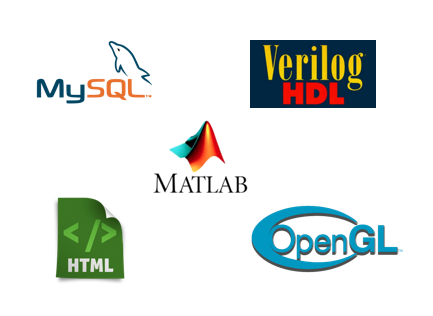
\includegraphics[scale=0.7]{images/A_DSLexamples}
\caption{Domain Specific Languages' Examples.}
\label{fig:A_DSLexamples} 
\end{figure}


\subsection{Binary Translation}\textit{}
\textbf{Binary translation} \textbf{\textit{(BT)}} is the process of \textbf{translating binary code} from one instruction set (\textbf{source architecture}) to another (\textbf{target architecture}) with the purpose of running an already compiled source code from the source architecture in a target platform (no need for code recompilation or modification). \cite{BinaryTranslation} 

Among several features, \textit{BT} can be used to reduce non-recurring engineering \textit{(NRE)} costs when achieving binary compatibility. \cite{DBT1}
Also, since the source and target \textit{ISA} can be the same, testing and debugging features can be provided, such as instruction trace and conditional breakpoints, allowing future \textbf{code optimization}. \cite{DBT1}

Most binary translation systems currently in use consists in migration tools which aid the transition from old architectures to newer ones. \cite{BinaryTranslation} Another encouragements for the use of binary translators are, e.g., in situations where the compilation of the source code to the target platform or instruction set is not available (or technically problematic) or when the source code is not available anymore. 

There are two main types of binary translators: \textbf{Static Binary Translator} and \textbf{Dynamic Binary Translator}. Their use in specific applications is determined by their own characteristics, as it will be shown next. 

\subsubsection{Static \textit{}Binary Translation}

In \textbf{static binary translation \textit{(SBT)}}, the \textbf{whole source binary code is translated} into code that runs on the target platform without having to run the code first. In this technique, the binary translation is performed statically, meaning, prior to system booting. \cite{DBT1}

The major problems related to this approach are caused by the fact that translation occurs in compile time. By so, not all the code can be discovered by the translator since there are situations where the execution flow is only known at run-time (e.g., indirect branches). Despite that, \textit{SBT} has several advantages since it allows performing more aggressive optimizations, which could yield more compact code and better code quality. It also avoids the translation overhead at run-time, being a good candidate for system with critical time constraints and resources. \cite{Shen:2014:RSB:2639036.2629335}

Some examples of applications that uses \textit{SBT} are:
\begin{itemize}
  \item In 2014, an \textbf{\textit{ARM} architecture} version of the 1998 video game \textit{StarCraft} was generated by \textbf{static} recompilation. 
  \item The \textbf{\textit{NES-to-x86}} statically recompiled version of the videogame \textit{Super Mario Bros}.
  \item The development of a tool to generate "C" code from \textit{GameBoy} binary that could then be compiled for a new platform, by Scott Elliott and Phillip R. Hutchinson from \textit{Nintendo} (2004). \cite{BinaryTranslation_example} 
\end{itemize}


\subsubsection{Dynamic Binary Translation}
In \textbf{dynamic binary translation (\textit{DBT})}, the source code is translated \textbf{on the fly} (dynamically) and cached in memory after being executed. In this technique, an intermediate layer between the source code and the execution platform is created in run-time, dedicated to translate and execute short sequences of code, referred as \textbf{basic blocks \textit{(BB)}}. \cite{DBT1} A basic block can be defined as a sequence of instructions with  a continuously flow of execution, which ends in a control flow instruction (e.g. branch instructions).

Executions performance under dynamic translation is achieved by balancing the cost of translation against the performance gains from translation. \cite{BinaryTranslation2} The major disadvantage of this technique is the overhead added to the execution (since the translation is performed every time a code block is fetched for the first time). Many applications are focused in the improvement of this problem via code optimization. This problem can also be amortized in application where code sequences are executed multiple times (diluting the translation time). Nonetheless, DBT has many advantages that overcomes the problems already identified in the SBT.     

Some examples of applications that uses \textit{DBT} are:
\begin{itemize}
  \item \textit{Apple} implemented a \textit{dynamic translating emulator }for M68K code in their \textit{PowerPC} line of \textit{Macintoshes}.
  \item \textit{Intel Corporation} developed an IA-32 Execution Layer - a \textit{DBT} designed to support IA-32 applications on \textit{Itanium}-based systems.
  \item Run-time optimizations to improve the performance of native binaries (\textit{Dynamo} and \textit{Mojo})
  \item Comprehensive performance measurements, profiling, memory analysis and debugging (\textit{Valgrind})
  \item Full machine virtualization (\textit{VMWare}). \cite{BinaryTranslation2}
\end{itemize}